\documentclass{report}
\usepackage[spanish]{babel}
\usepackage[utf8]{inputenc}
\usepackage{graphicx}
\usepackage{amssymb, amsmath} %Paquetes matemáticos de la American Mathematical Society
\begin{document}
	%Portada
	\begin{titlepage}
		%
\includegraphics[width=0.2\textwidth]{ipn}
		%
\includegraphics[width=0.3\textwidth]{escom}
		\begin{center}
			\bfseries\LARGE Instituto Politécnico Nacional \par
			\bfseries\LARGE Escuela Superior de Cómputo \par
			\vspace{3cm}
			\scshape\large PRACTICA 1: DETERMINACIÓN EXPERIMENTAL DE LA COMPLEJIDAD TEMPORAL DE UN ALGORTIMO \par
			\vspace{1cm}
			\large Tejeda Moyao Leon Francisco \par
			\itshape\large leontejeda@gmail.com \par
			\vspace{1cm}
		\end{center}
		
		
		\begin{bf}
			\large Resumen:
		\end{bf}
	
		\large En la presente practica, la tarea fue desarrollar 2 algortimos.\par
		\begin{itemize}
			\item Encontrar un valor repetido en un arreglo.
			\item Elaborar el algoritmo de euclides.
		\end{itemize}
			
		\bf\large Palabras Clave: Complejidad, Algoritmo, C \par
		
		\vfill
	\end{titlepage}

	\section* {Introducción.}
	\large 
	\begin{itemize}
		\item
		\begin{bf}
			\large Importancia de de los algortimos. \par
		\end{bf}
	
		\large Los algoritmos se pueden definir como una sucesión de pasos que se deben de seguir para desarrollar una tarea dada. \par
		\large Por lo tanto se podría decir que la importancia de los algoritmos radica en que al momento de deifnir un algoritmo, este puede implemnmetarse en uno o varios problemas y, de cierta manera, es mas facil resolver ciertos problemas. \par
	
		\item
		\begin{bf}
			\large Importancia de analizar un algoritmo. \par
		\end{bf}
		
		\large Al momento de analizar un algoritmo, se puede llegar a saber el número de pasos que realiza y/o el número de tiempo que le toma llegar al resultado deseado. \par
		\begin{bf}
			\large NOTA: Que el codigo del algortimo sea mas pequeño, no significa que tarde menos tiempo) \par
		\end{bf}
		\large Independientemente de lo que se requira analizar, analizando el algortimo se puede llegar a saber en que parte el algoritmo puede moejorar para asi ahorrar recursos, ya sea en tiempo o memoria. \par
	
		\item
		\begin{bf}
			\large Objetivo. \par
		\end{bf}
	
		\large Realizar el analisis a postereori de ambos codigos realizados y ver sus graficas en el programa demos. \par
	\end{itemize}
	
	
	\section* {Conceptos Básicos.}
		\begin{itemize}
			\item
			\begin{bf}
				\large Algortimo. \par
			\end{bf}
		
			\large Secuencia de pasos o insturcciones, meidante las cuales se llegar a realizar una tarea. \par
		
			\item
			\begin{bf}
				\large Complejidad Algoritmica. \par
			\end{bf}
		
			\large Se traduce como la descripción de un algortimo en cuanto a tiempo de ejecución y memoria requerida. \par
		
			\item
			\begin{bf}
				\large Analisis Apostereori. \par
			\end{bf}
		
			\large Es el anilisis de un algortimo despues de que este ha sido ejecutado, recolectando la información obtenida durante su ejecución. \par
			
		\end{itemize}
	
	\section* {Experimentación y Resultados.}
	\large Para el primer algoritmo, se encargó que en un arreglo de tamaño N se llenara con valores aleatorios que fueran desde 1 hasta 3N, posteriormente este arreglo de dividiria en 2 partes. Finalmente se buscará un valor repetido en ambas mitades del arreglo, cuando encuentre un valor repetido el programa finalizara. \par
	\begin{figure}[h]
		\centering
		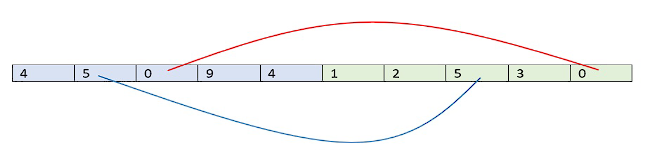
\includegraphics[width=0.8\textwidth]{1} \par
		\caption{Ejemplo arreglo.}
	\end{figure}

	\large Habiendo corrido el algoritmo, este imprime los valores obtenidos, indica los valores ingresaados y termina indicando si encontró el valor y en que posición. \par
	\begin{figure}[h]
		\centering
		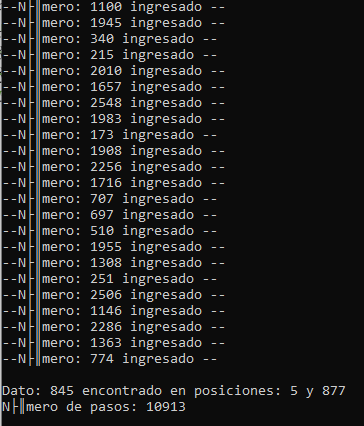
\includegraphics[width=0.4\textwidth]{2} \par
		\caption{Funcionamiento primer algortimo.}
	\end{figure}
	
	\newpage
	
	\large El número de pasos y el tamaño del arrelgo son guardados en un archivos con extensión .csv. En la primera columna será el tamaño y en la segunda el número de pasos.\par
	\begin{figure}[h]
		\centering
		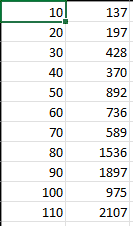
\includegraphics[width=0.2\textwidth]{3} \par
		\caption{Datos programa 1.}
	\end{figure}

	\large Se hizo uso del programa desmos, el cual permite mostrar la gráfica obtenida, esta se obtiene pegando los datos del archivo .csv.\par
	\begin{figure}[h]
		\centering
		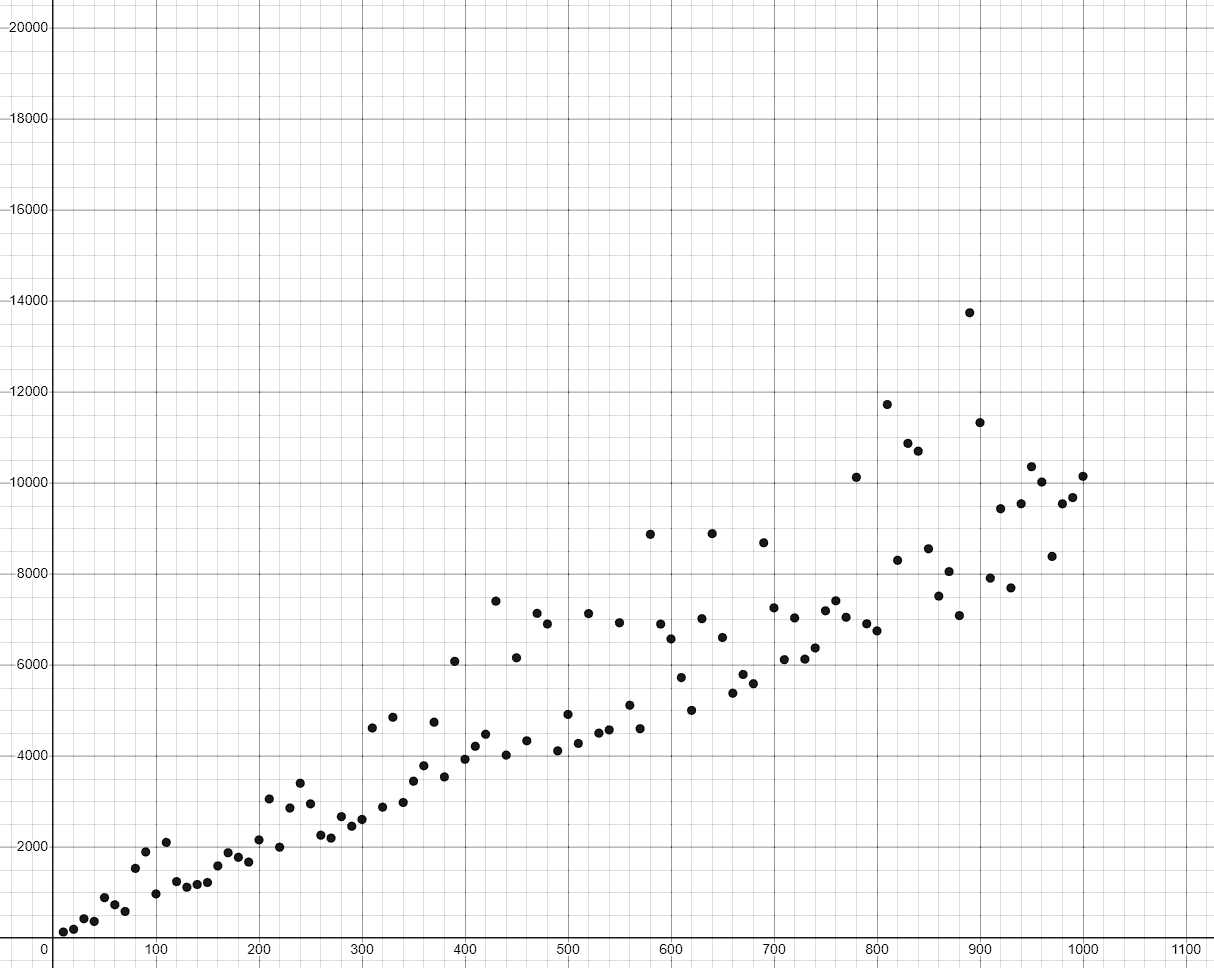
\includegraphics[width=0.6\textwidth]{4} \par
		\caption{Gráfica programa 1.}
	\end{figure}

	\large Se buscó tanto la cota superior como la cota inferior y se procedió a comprobar si la función estab aaoctada por dichas funciones.\par
	
	\newpage
	
	\begin{itemize}
		\item\bf Cota Superior: $\Omega$ (1) \par
		\item\bf Cota Inferior:	$\mathcal{O}$  (N^2) \par
	\end{itemize}

	\begin{figure}[h]
		\centering
		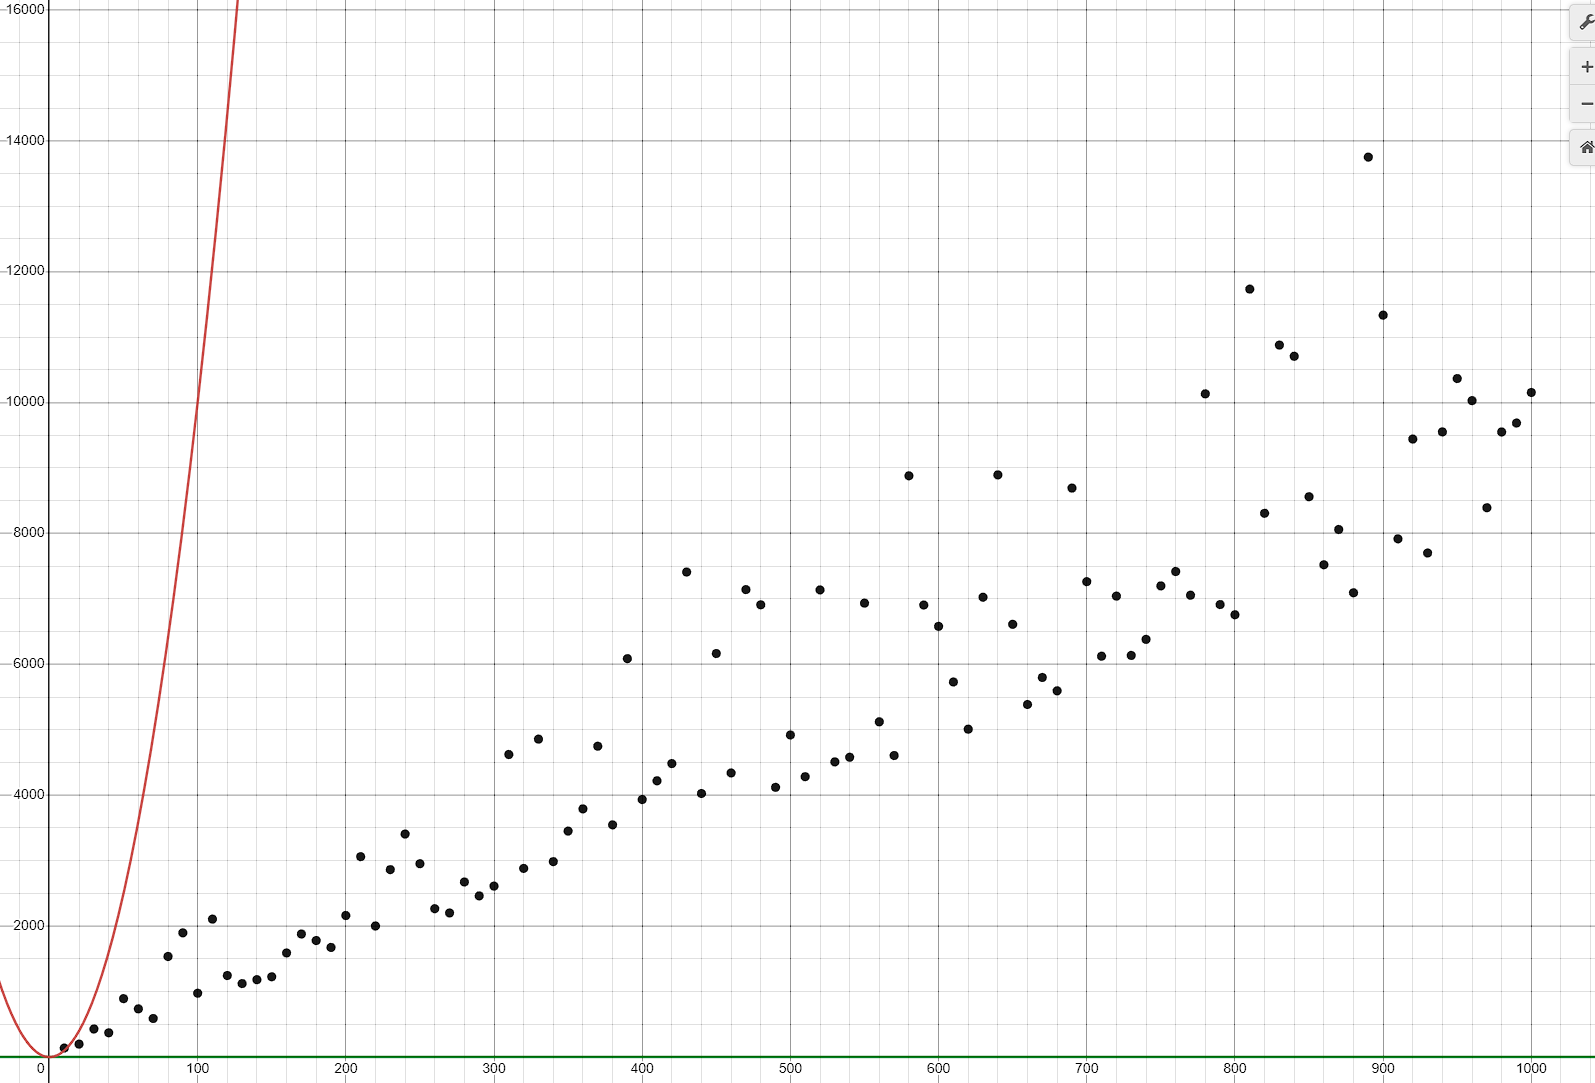
\includegraphics[width=0.6\textwidth]{5} \par
		\caption{Gráfica programa 1 con cotas.}
	\end{figure}
	
	
	
	\section* {Conclusiones.}
	\large En esta practica se usaron herramientas que ayudarón a la interpretación del comportamiento del código, esto gracias a los datos que fueron guardados y almacenados en los archivos con extensión .csv. \par
	\large Durante el desarrollo de esta se pudo observar que en el primer caso se podia mejorear el algortimo, al solo recorrer la mitad del arreglo en los ciclos implementados en vez de recorrer todo el arreglo.
	
	\begin{bf}
		Conclusiones Alumno 1: 
		
\includegraphics[width=0.15\textwidth]{alumno} \par
	\end{bf}
	\large En la practica se pudo visualizar el comportamiento del algortimos que fue utilizado, esto nos ayudó a poder visualizar una mejor manera de ocmo realizar el mismo trabajo con menor tiempo simplemente modificando el algortimo solo un poco. \par
	
	%\section* {Anexo.}
	
	%\section* {Bibliografía.}
	
	
\end{document}